Afin de mettre en place nos classifieurs pour identifier les nuages de points 3D, nous avons tout d'abord dû extraire plusieurs métriques nous permettant de représenter nos images de points. Nous prenions pour cela en entrée un fichier par nuage de points, comportant pour chaque point ses coordonnées (x, y et z) et son intensité. Voici en figure \ref{fig:nuage_de_points} un exemple de nuage de points représentant un cycliste :

	\begin{figure}[H]
		\centering
		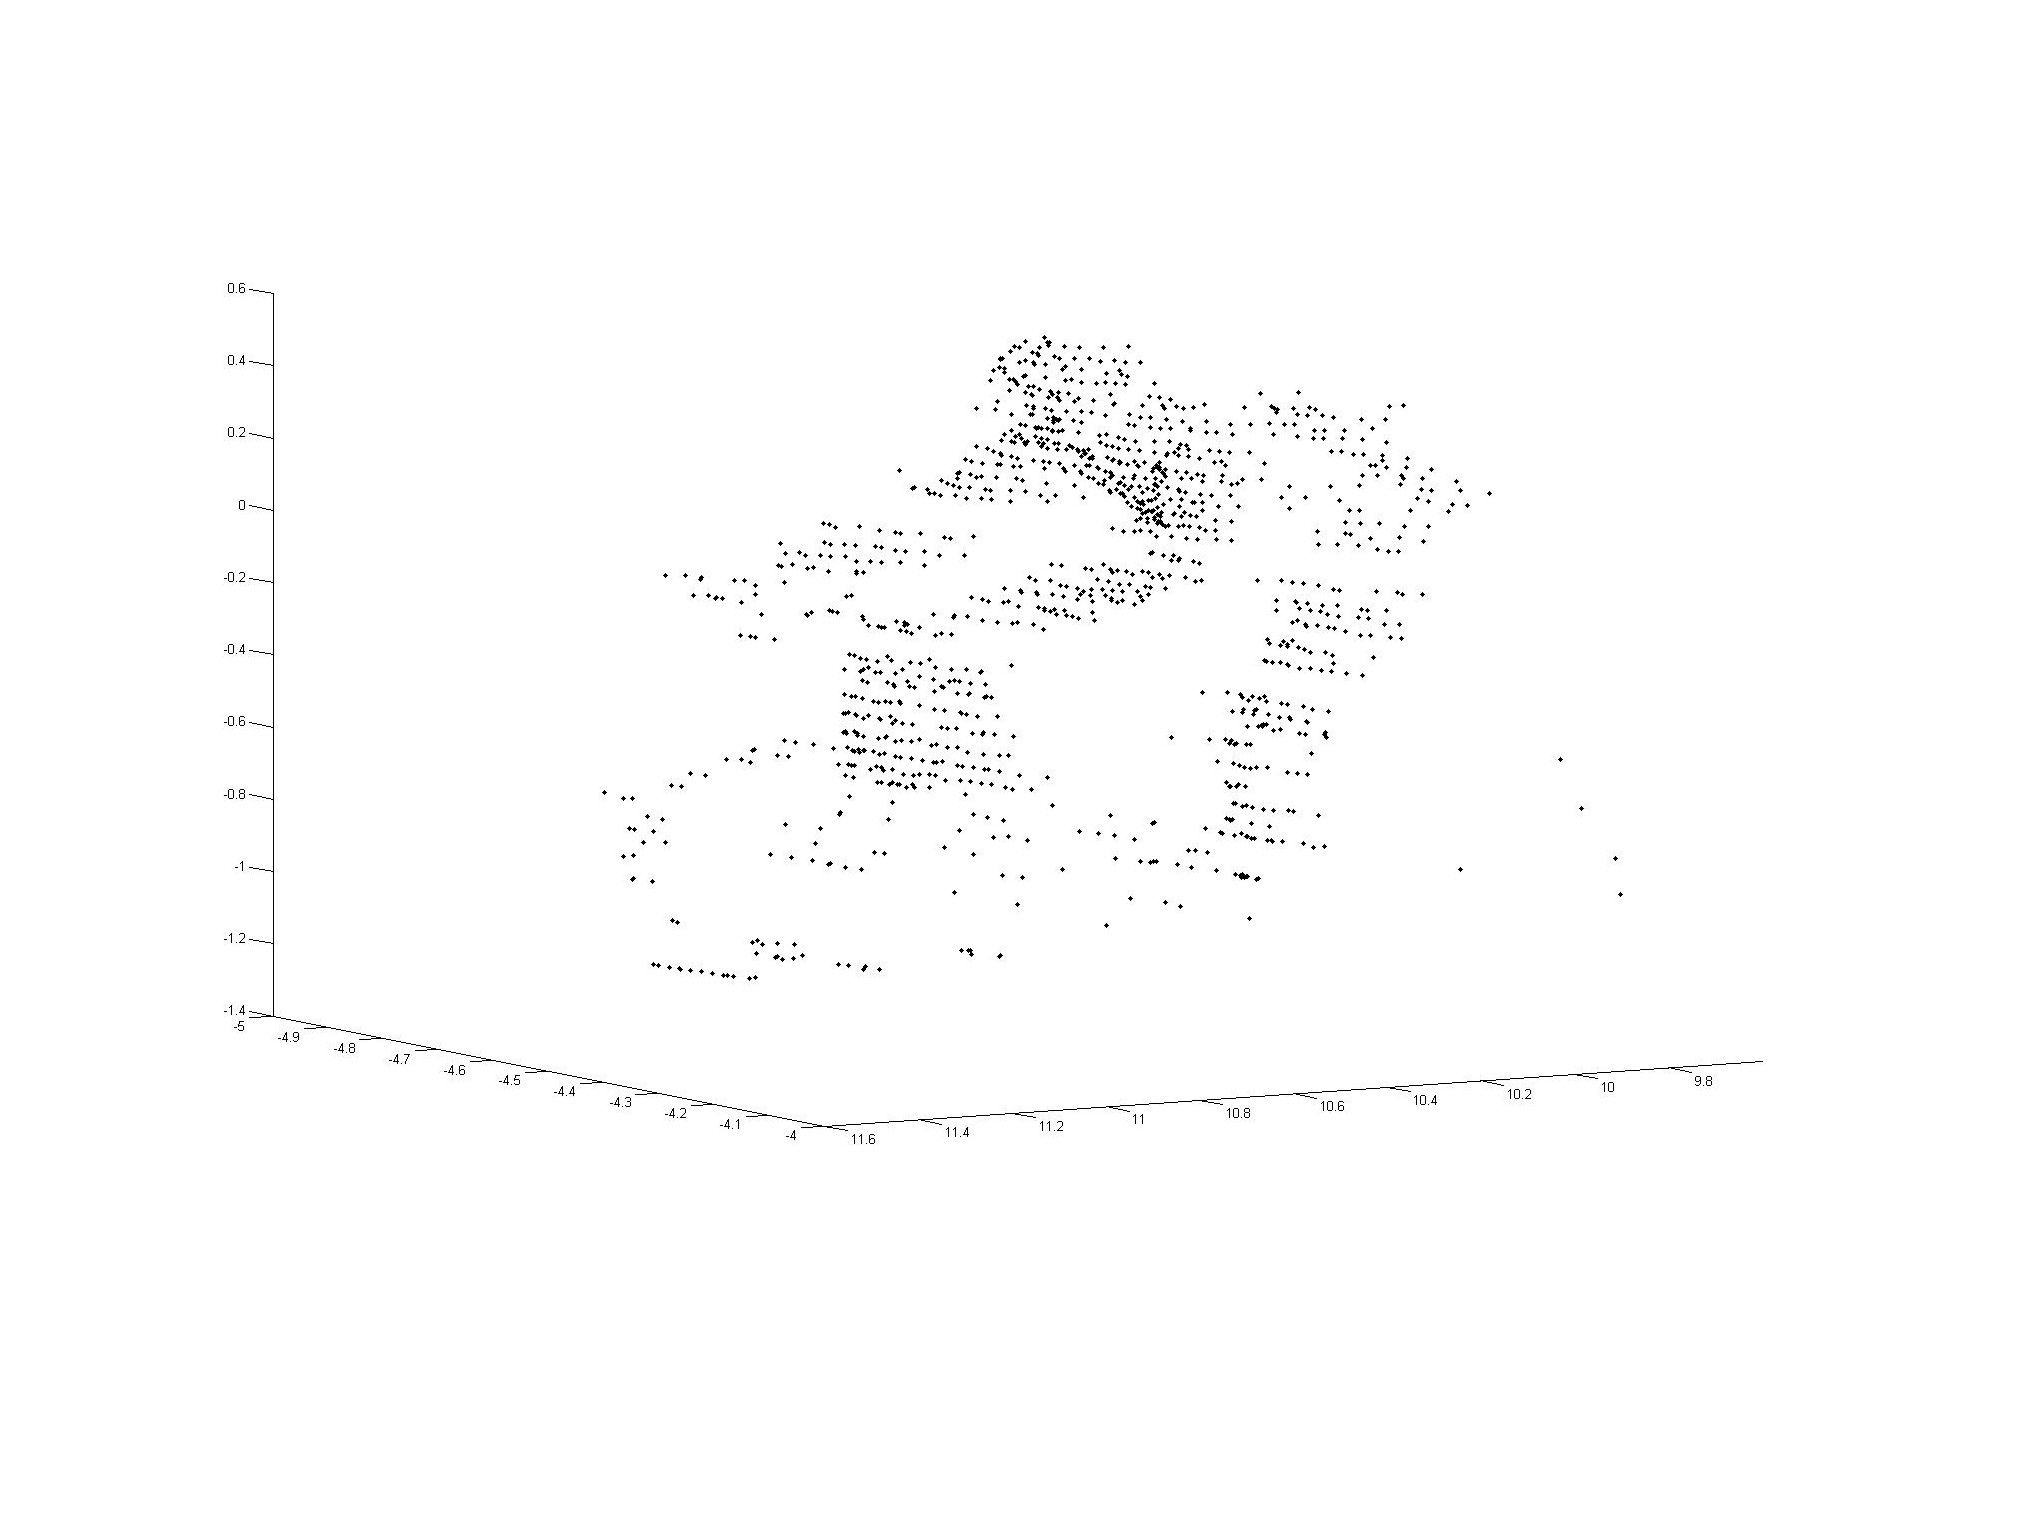
\includegraphics[scale=0.25]{images/objet3D2.jpg}
		\caption{Exemple de \emph{nuage de points}}
		\label{fig:nuage_de_points}
	\end{figure}

\section{Attributs utilisés}
	\subsection{Métriques statistiques basiques}
		Dans un premier temps, nous avons extrait des métriques statistiques très simples basées sur l'intensité des points. Nous avons pour chaque nuage de points calculé la moyenne, la variance, le minimum et le maximum des intensités.\\

		En effet, ces valeurs changent selon les classes. On peut le voir dans le tableau suivant, présentant les moyennes des quatre attributs sur des nuages de points de type voitures et background :\\

		\begin{center}
			\begin{tabular}{|l||c|c|c|c|}
			  \hline
			  & Minimum & Maximum & Moyenne & Variance \\
			  \hline
			  Voitures & 34.5 & 249 & 120 & 3500 \\
			  Background & 48.7 & 196 & 125 & 1548 \\
			  \hline
			\end{tabular}
		\end{center}


		Cela nous montre que ces attributs peuvent présenter des différences significatives selon les classe, il est donc intéressant de prendre en compte ces métriques pour la classification.

	\subsection{Bounding-box}
		La \emph{bounding-box} permet de connaître la forme de l'objet en 3D pour distinguer des objets de catégorie différentes.

		\begin{figure}[H]
			\centering
			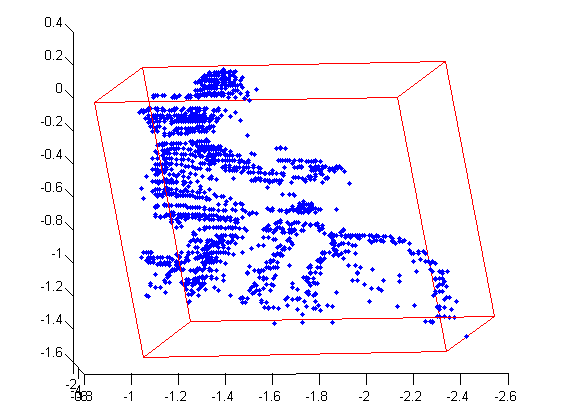
\includegraphics[scale=0.6]{images/bounding_box_cyclist_2.png}
			\caption{Exemple de \emph{bounding-box} sur un cycliste}
			\label{fig:image}
		\end{figure}

		La \emph{bounding-box} représente l'amplitude du nuage de points selon les trois dimensions. Pour chaque dimension, nous aurons donc un attribut qui correspond à la différence entre le maximum de cette coordonnée et le minimum de cette coordonnée, pour chaque nuage de points.\\

		Afin de pouvoir calculer la \emph{bounding-box}, nous avons dû "redresser" le nuage de points selon l'axe $z$, en considérant que le terrain est plat et qu'il n'y a donc pas besoin de redresser l'image selon $x$ et $y$).
		Nous avons donc calculé l'angle $\theta$ de la rotation, grâce à la formule:

		\[ tan(2 \theta) = 2 \times \frac{\bar{x}\bar{y}}{\bar{x}^2 - \bar{y}^2} \]
		\[ \theta = \frac{1}{2} \times arctan(2 \frac{\bar{x}\bar{y}}{\bar{x}^2 - \bar{y}^2}) \]

		avec \[ \bar{x} = \frac{1}{n} \times \sum_{i =1}^n{x_i} \]
		\[ \bar{y} = \frac{1}{n} \times \sum_{i =1}^n{y_i} \]

		Une fois que nous avons trouvé l'angle de rotation, il faut appliquer la rotation au nuage de points. Pour cela on construit la matrice $R_z$ telle que :

		\[\begin{bmatrix}
		   cos(\theta) & -sin(\theta) & 0 \\
		sin(\theta) & cos(\theta) & 0 \\
		0 & 0 & 1
		\end{bmatrix}\]

		On calcule ensuite le nouveau nuage de points redressé avec la formule:
		\[ P_T = R_z \times P_0\]
		où $P_0$ est le nuage de points d'origine. \\

		Nous appliquons ensuite une translation à l'origine sur le nuage de points redressé pour le centrer. On peut maintenant calculer les 3 attributs de la \emph{bounding-box} sur ce nouveau nuage de points.


	\subsection{Scatter-ness, linear-ness et surface-ness}
		D'autres attributs intéressants à étudier dans le cadre de la reconnaissance d'objets 3D sont la \emph{scatter-ness}, la \emph{linear-ness} et la \emph{surface-ness}, qui traduisent la forme de l'objet.

		Pour les calculer, on calcule tout d'abord la matrice de covariance des coordonnées des points, puis on calcule les valeurs propres $\lambda_0$, $\lambda_1$ et $\lambda_2$ de la matrice de covariance. \\

		On s’intéresse ensuite à la différence entre ces valeurs :
		\begin{itemize}
			\item Si ces trois valeurs sont similaires ($\lambda_0 \approx \lambda_1 \approx \lambda_2$), les points sont répartis de manière égale selon les trois dimensions, comme pour une sphère. On dit qu'ils sont dispersés et on parle de \emph{scatter-ness}.
			\item Si au contraire une valeur est beaucoup plus grande que les deux autres ($\lambda_0 \gg \lambda_1 \approx \lambda_2$), cela signifie que les points sont principalement répartis sur une seule dimension, ils forment une sorte de ligne. On parle alors de \emph{linear-ness}.
			\item Si une valeur est beaucoup plus petite que les deux autres ($\lambda_0 \approx \lambda_1 \gg \lambda_2$), cela signifie que les points sont répartis sur deux dimensions, et forment quasiment une surface. On parle alors de \emph{surface-ness}.\\
		\end{itemize}

		Nous allons donc nous intéresser aux attributs suivants :
		\begin{itemize}
			\item $\lambda_0$, qui représente la \emph{scatter-ness};
			\item $\lambda_0 - \lambda_1$, qui représente la \emph{linear-ness};
			\item $\lambda_1 - \lambda_2$, qui représente la \emph{surface-ness};
		\end{itemize}

\section{Attribut étudié : les spin-images}

	La spin image est l’image du nuage 3D prise en un point, perpendiculairement à la normale en ce point (donc selon le plan tangent). Le but est de prendre les meilleures spin images pour chaque nuage de points car c’est sur ces images 2D que nous pouvons réaliser une classification.


\section{Autre attribut possible : les images orthogonales}

	Les images orthogonales sont obtenues par projection orthogonale de l'image 3D. La projection orthogonale se fait selon une direction de projection, sur un plan tel que le plan et la direction sont orthogonaux. Il n'y a donc pas de point de vue. Des caméras existent afin de récupérer directement ces images, à l’opposition des caméras classiques qui capturent la projection en perspective de l'objet, de la même manière que l’œil humain. Ces images peuvent ensuite être utilisées pour réaliser la classification.

